\documentclass[print]{vakidioot}

\genre   {Column}
\title   {Waarom Informatiekunde \mbox{eigenlijk net Friesland is}}
\subtitle{En andere domme vergelijkingen}
\author  {Chun Fei Lung}

\begin{document}
    \dummypagina

    \begin{wrapfigure}[0]{r}{3.9cm}
        \vspace{.55cm}
        \includegraphics[width=3.9cm]{Friese-Vlag-(niet-die-van-de-zuivel)}
    \end{wrapfigure}
  
    \maketitle

    \begin{lead}
        Informatiekunde kampt onder veel bèta's een beetje met een imagoprobleem. Buiten de informatiekundigen zelf weet vrijwel niemand wat het inhoudt, laat staan wat het te zoeken heeft bij een exactestudiesclubje als \aesnaam. Wat dat betreft is Informatiekunde enigszins vergelijkbaar met Friesland. Dat klinkt misschien raar, maar het is best wel logisch als je er een minuutje over nadenkt.\footnote{Maar ook niet langer dan een minuut, want dan kom je geheid tot de conclusie dat studierichtingen en provincies totaal andere dingen zijn, en je dus net zo goed appels met beren kunt vergelijken (maar dat gaan we volgend nummer pas doen, anders denkt iedereen dat ik geen leven heb).}
        % Ja, ik bedoel hier echt beren, want appels en peren hebben nog best veel met elkaar gemeen
    \end{lead}
  
    \begin{multicols}{2}
        Omdat het belangrijk is dat je niet (te veel) over die ene minuut heen gaat, zal ik zo weinig mogelijk tijd verkwisten aan paginavullende onzin als argumentatie, maar me beperken tot kant en klare brokken \textit{truthy} feitjes. Hopelijk bereik je dan ook netjes binnen de tijd het einde van de volgende pagina.
    
        \section*{\vspace{-.5\baselineskip}Natuur- en Sterrenkunde}
        Als ik nu vertel waarom Informatiekunde eigenlijk net Friesland is, stop je waarschijnlijk direct met lezen, dus ik begin eerst met Natuur- en Sterrenkunde, want dat is iets dat absoluut geen Informatiekunde is. En ik kan het weten, want ik begrijp op Vakidiootvergaderingen geen drol van waar de rest van de overwegend natuurkundige -- en wiskundige, maar laten we het daar nog niet over hebben -- redactie het over heeft.
        
        Ook hebben beide studies debiele zusjes waar ze nogal eens mee verward worden. Voor Informatiekunde is dat Informatiewetenschappen, wat erg dicht tegen de communicatiewetenschappen aan zit\footnote{Om het wel even goed verwarrend te houden: Informatiekunde is in het Engels \textit{information science}, en als je dat letterlijk vertaalt naar het Nederlands, krijg je dus inderdaad\ldots{} informatiewetenschap.}. Sterrenkunde heeft het nog een stukje slechter, die heeft namelijk Astrologie als debiel zusje.

        \begin{pullquote}
          Q: How do you know\\ if there is a Frisian at the dinner table?\\
          A: Don't worry, (s)he'll tell you about it.
        \end{pullquote}
        
        Maar we gaan weer even terug naar hét verschil tussen Natuur- en Sterrenkunde en Informatiekunde: die eerste kent iedereen wel, die tweede niemand.\\
        Vraag een niet-bèta om een bètastudie te noemen, en hij/zij komt niet verder dan Natuur- of Sterrenkunde -- velen zullen zelfs denken dat ze gewoon heel bèta zijn. Daarmee zijn Natuur- en Sterrenkunde dus net Noord- en Zuid-Holland: daarvan denken mensen ook dat dat heel Nederland is. Overigens is dat ook een beetje onze schuld, want als het ons toevallig beter uitkomt, roepen we ook met zijn allen dat we Hollanders zijn. % NNV, te subtiel?
        
        \section*{Wiskunde}
        Als er, naast Engels, \textit{iets} is dat zo'n beetje alle bètawetenschappen verbindt, dan is het wel de wiskunde.
        
        Puur om deze reden zouden we al kunnen zeggen dat Wiskunde Utrecht is. Dat verbindt namelijk een groot deel van Nederland met elkaar.\\
        Daarnaast is Utrecht -- vooral in de spitsuren -- óók niet zo heel toegankelijk voor mensen die er niet zo bekend mee zijn, en de meeste Nederlanders zouden het dus het liefst compleet vermijden als dat niet nóg onpraktischer zou zijn geweest.
        
        \section*{Informatica}
        Van de \aesnaam{}studies is Informatica de meest praktijkgerichte, en de enige waarvan buitenstaanders niet constant roepen dat je er niks aan hebt.\\
        Dat is ergens best wel raar, want waar Natuur- en Sterrenkunde bijvoorbeeld onderzoekt hoe de echte wereld werkt, leven de informatici gewoon in hun eigen wereldje met hun harde waar-óf-onwaar-waarheden.
        
        Afgezien daarvan vind ik informatici heel aardige mensen hoor, al lijkt het er vaak op dat ze allemaal net wat andere talen gebruiken, wat soms een beetje lastig communiceert. Datzelfde gevoel heb ik trouwens ook als ik mensen uit Noord-Brabant spreek.
        
        \section*{Die andere studies}
        Er zijn nog heel veel meer b\`etastudies buiten de paar die \aesnaam onder zich heeft, maar omdat ze retesaai zijn, willen we nog wel eens vergeten dat ze bestaan. Net als Gelderland, Overijssel, Zeeland, Groningen, Limburg, en Dinges.

        \columnbreak
        
        \section*{\vspace{-1.5\baselineskip}Informatiekunde}
        En dan hebben we dus nog Informatiekunde. Dat is een soort toegepaste informatica, wat op zijn beurt eigenlijk een soort toegepaste wiskunde is (wat informatiekunde overigens nog geen toegepaste toegepaste wiskunde maakt).
        
        Met haar \textit{roots} in de sociale wetenschappen, de geesteswetenschappen, de bedrijfskunde, en de informatica, heeft Informatiekunde een grotendeels compleet andere achtergrond dan de andere \aesnaam{}studies. Daarmee zit er dus een flinke kloof tussen de drie eerder genoemde studies en Informatiekunde -- dit geldt uiteraard net zo goed voor Friesland, dat ook teringver weg ligt van het relevante deel van Nederland.
        
        Nu zullen sommige lezers wel denken, ,,\textit{Heel leuk en aardig, maar Groningen ligt toch echt verder weg dan Friesland hoor}''. Als je kijkt op de kaart, dan ligt Groningen (dat ooit trouwens ook Fries was) inderdaad verder weg. Maar Groningen heeft tenminste nog wél als \textit{redeeming quality} dat het door de aardschokken veelvuldig op televisie komt, waardoor het toch dichterbij lijkt.

        \section*{Tot slot}
        Er is nog één provincie die ik niet heb genoemd, en dat is Flevoland: Die bewaar ik voor later, als er een nieuwe studierichting komt waarvan je niet eens meer kan zeggen dat `ie nog met één been in bètaland staat. Iets als Toegepaste Informatiekunde misschien. Kunnen we daar weer op zeiken.
    \end{multicols}
    
    \enlargethispage{\baselineskip}
    
    \begin{figure}[t]
      \centering
      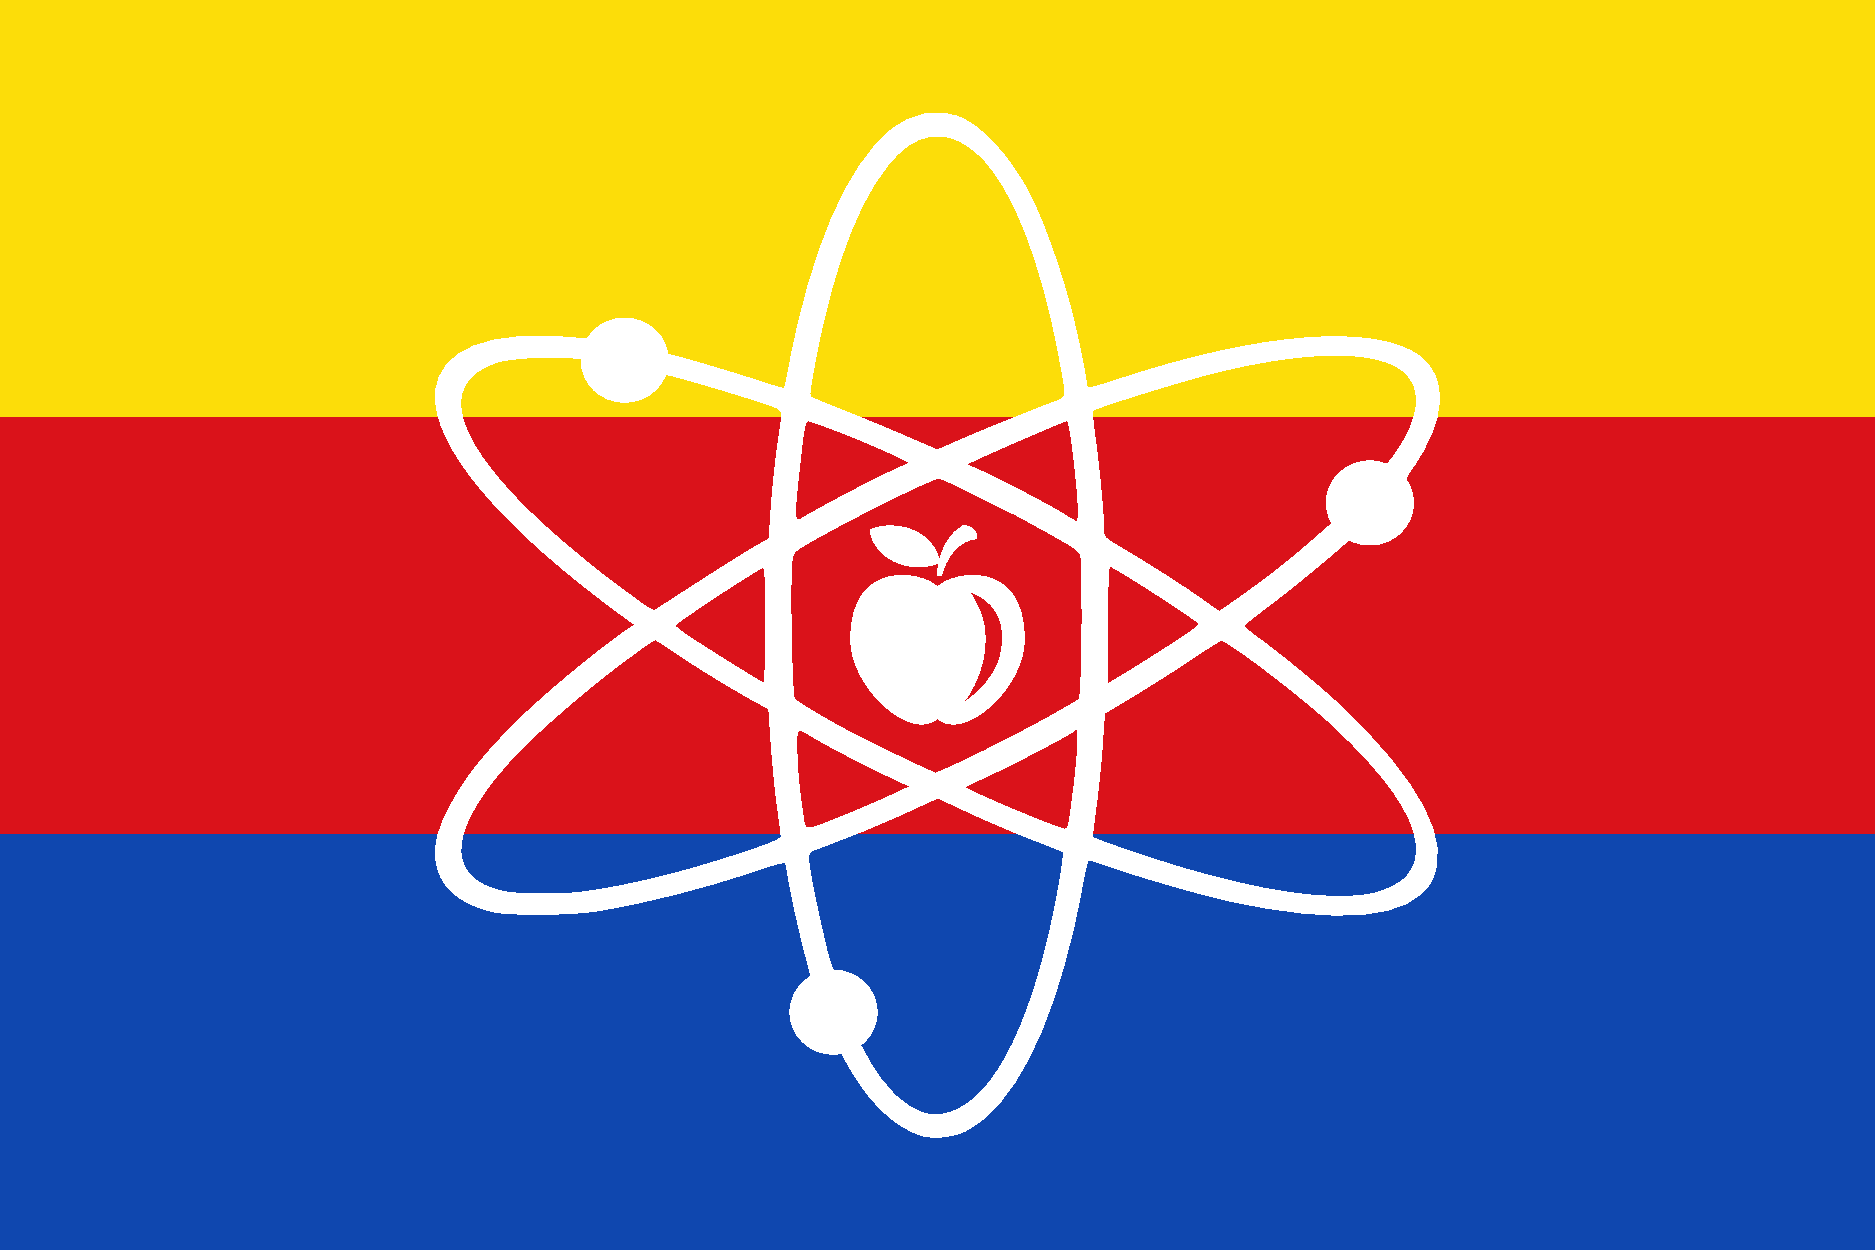
\includegraphics[width=.24\columnwidth]{Noord-Holland.pdf}
      \hfil
      
\includegraphics[width=.24\columnwidth]{Zuid-Holland.pdf}
      \hfil
      
\includegraphics[width=.24\columnwidth]{Utrecht.pdf}
      \hfil
      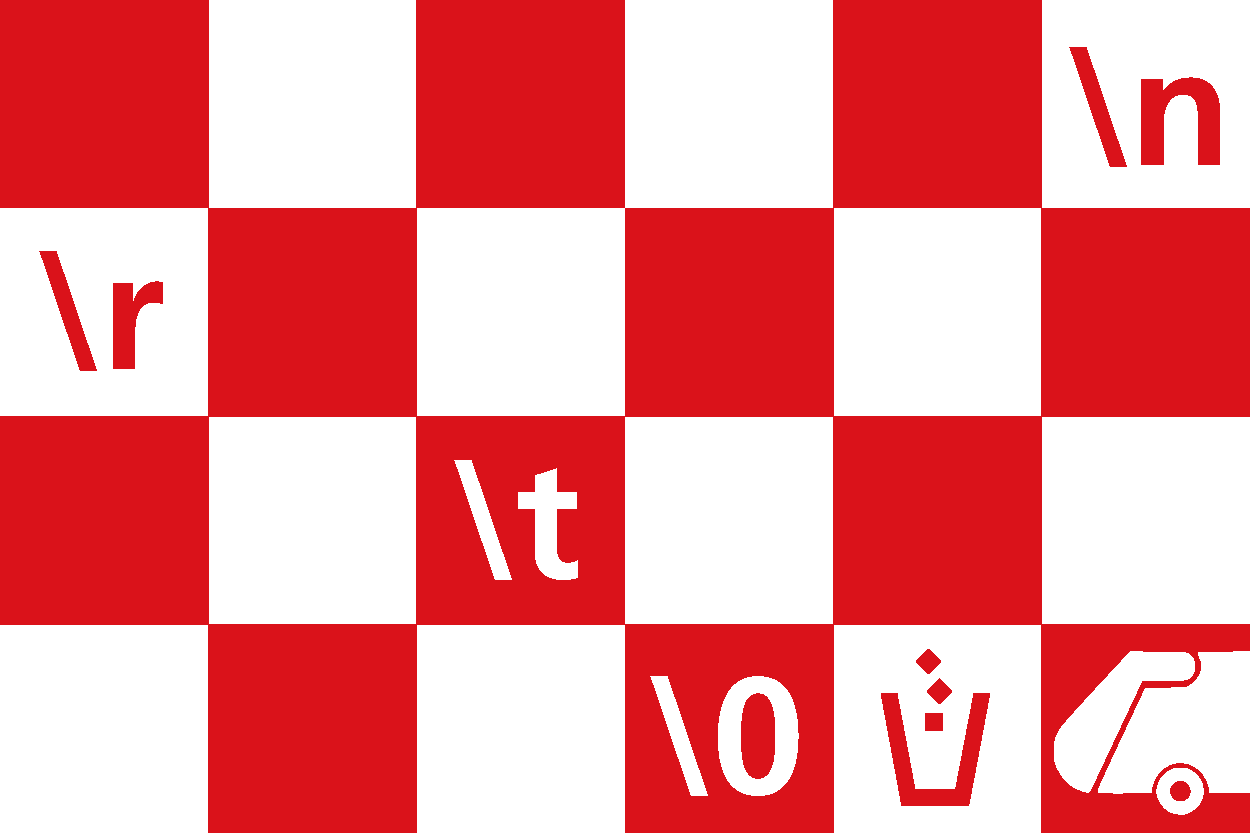
\includegraphics[width=.24\columnwidth]{Noord-Brabant.pdf}
      \caption*{Van links naar rechts: Friesland, Noord-Holland, Zuid-Holland, Utrecht, en Noord-Brabant}
    \end{figure}
\end{document}
